Im Folgendem werden die für den Versuch benötigten Fourierkoeffizienten
der in den Abbildungen \ref{fig:Aufgaben_Rechteck} bis \ref{fig:Aufgaben_Sägezahn} dargestellten Spannungen 
berechnet.
	\begin{figure}[h!]
		\centering
		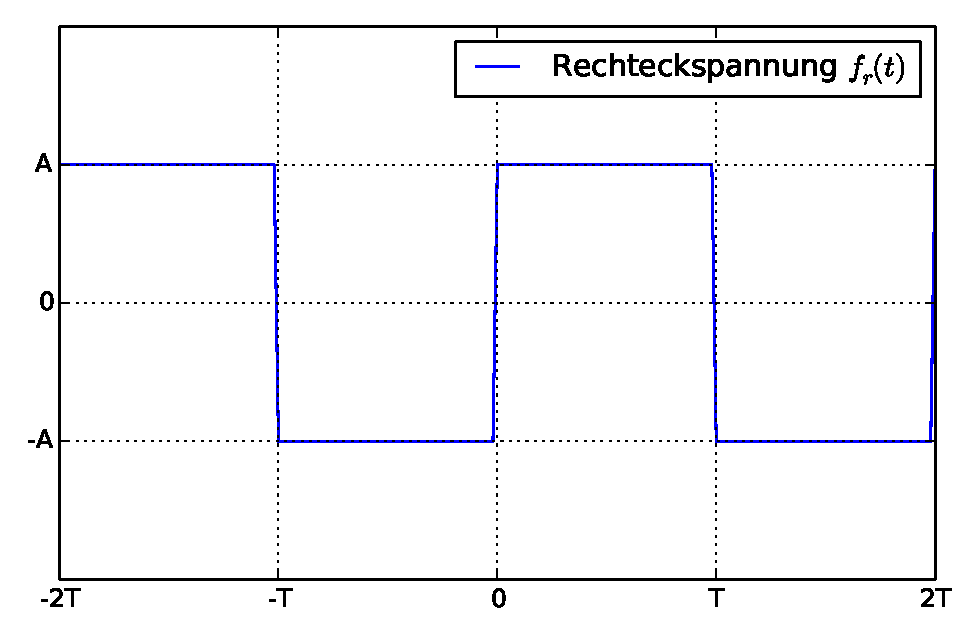
\includegraphics[scale=0.35]{Grafiken/RechteckSpannung.pdf}
		\caption{Für die Berechnung genutzte Rechteckspannung}
		\label{fig:Aufgaben_Rechteck}
	\end{figure}
	
	\begin{figure}[h!]
		\centering
		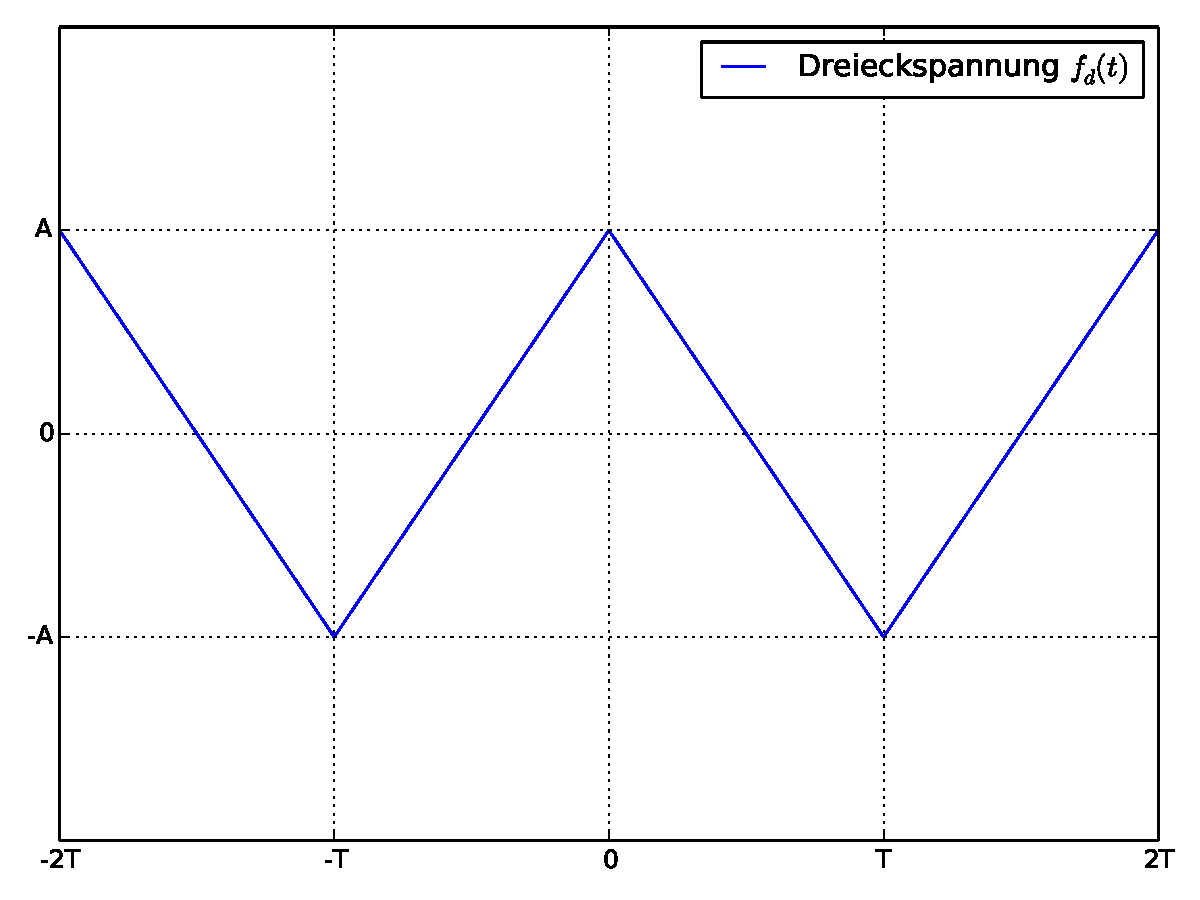
\includegraphics[scale=0.35]{Grafiken/DreieckSpannung.pdf}
		\caption{Für die Berechnung genutzte Dreieckspannung}
		\label{fig:Aufgaben_Dreieck}
	\end{figure}
	

	\begin{figure}[h!]
		\centering
		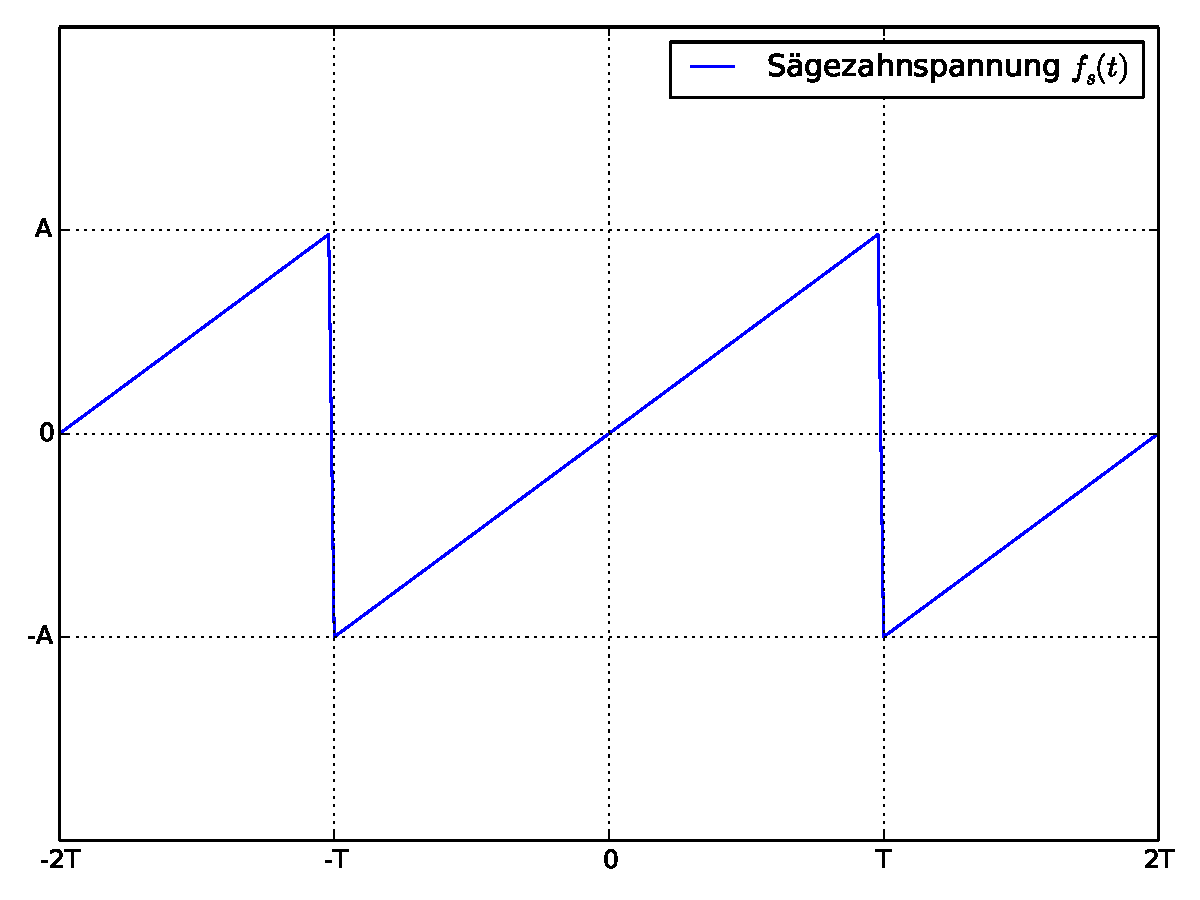
\includegraphics[scale=0.35]{Grafiken/SaegezahnSpannung.pdf}
		\caption{Für die Berechnung genutzte Sägezahnspannung}
		\label{fig:Aufgaben_Sägezahn}
	\end{figure}

\subsection{Rechteckspannung}

	Die Fourierkoeffizienten der in \cref{fig:Aufgaben_Rechteck} dargestellten Spannung
	mit der Definition
	\begin{empheq}{equation}
		f_{r}(t) = \begin{cases}
					- A\ &, \ - T < t < 0\\
					  A\ &, \ 0 < t < T 	
				\end{cases}
	\end{empheq} 
	berechnen sich zu:
	\begin{empheq}{align}
		a_{0} &= \dfrac{1}{T} \int\limits_{-T}^{T} f(t) \dif t = 0,\ \text{da}\ f(t)\ \text{ungerade}\\
		a_{n} &= \dfrac{1}{T} \int\limits_{-T}^{T} f(t) \cdot \cos(\frac{n\pi}{T} t) \dif t = 0,\ \text{da}\ f(t)\ \text{ungerade}\\
		b_{n} &= \dfrac{1}{T} \int\limits_{-T}^{T} f(t) \cdot \sin(\frac{n\pi}{T} t) \dif t \nonumber\\
		&= \dfrac{2}{T} \int\limits_{0}^{T} A \cdot \sin(\frac{n\pi}{T} t) \dif t \nonumber\\
		&= \dfrac{2A}{n\pi}   \sbr{-\cos(\frac{n\pi}{T} t)}_{0}^{T}  \nonumber\\
		b_{n} &= \dfrac{2A}{n\pi}   \sbr{1 - \cos(n\pi)}  = 
		\begin{cases}
			\dfrac{4A}{n\pi}\ &,\ n \mod{2} \neq 0\\
			0 \ &,\ n \mod{2} = 0
		\end{cases}  
	\end{empheq}
	
	
\subsection{Dreieckspannung}

		Die Fourierkoeffizienten der in \cref{fig:Aufgaben_Dreieck} dargestellten Spannung
		mit der Definition
		\begin{empheq}{equation}
			f_{d}(t) = A - \dfrac{2A}{T} \envert{t}\ , \ -T < t < T
		\end{empheq} 
		berechnen sich zu:
		\begin{empheq}{align}
			a_{0} &= \dfrac{1}{T} \int\limits_{-T}^{T} f(t) \dif t = 0,\ \text{in \cref{fig:Aufgaben_Dreieck} ersichtlich}\\
			b_{n} &= \dfrac{1}{T} \int\limits_{-T}^{T} f(t) \cdot \sin(\frac{n\pi}{T} t) \dif t = 0,\ \text{da}\ f(t)\ \text{gerade} 
		\end{empheq}
		\begin{empheq}{align*}
			a_{n} &= \dfrac{1}{T} \int\limits_{-T}^{T}  \del{A - \dfrac{2A}{T} \envert{t}} \cdot \cos(\frac{n\pi}{T} t) \dif t \nonumber\\
			&= \dfrac{2}{T} \int\limits_{0}^{T}  \del{A - \dfrac{2A}{T} t} \cdot \cos(\frac{n\pi}{T} t) \dif t \nonumber\\
			&= \dfrac{2A}{T} \del{ \underbrace{\int\limits_{0}^{T} \cos\!\del{\frac{n\pi}{T}t} \dif t}_{= 0}} - \dfrac{4A}{T^{2}} \del{  \int\limits_{0}^{T} t \cos\!\del{\frac{n\pi}{T}t}\dif t}  \nonumber\\      
			&= - \dfrac{4A}{T^{2}} \del{\underbrace{\sbr{\dfrac{Tt}{n\pi}\sin\!\del{\frac{n\pi}{T}t} }_{0}^{T}}_{= 0} - \dfrac{T}{n\pi} \int\limits_{0}^{T}  \sin\!\del{\frac{n\pi}{T}t}\dif t}  \nonumber\\      
			&= - \dfrac{4A}{T^{2}} \del{- \dfrac{T^{2}}{(n\pi)^{2}} \sbr{-\cos\!\del{\frac{n\pi}{T}t}}_{0}^{T}}  \nonumber\\      
			&= - \dfrac{4A}{(n\pi)^{2}} \del{\cos\!\del{n\pi} - 1}  \nonumber\\      
			\end{empheq}
			
			\begin{empheq}{align}
			a_{n} &=  \begin{cases}
					\dfrac{8A}{(n\pi)^{2}}\ &,\ n \mod{2} \neq 0\ \\
					0 &,\ n \mod{2} = 0 \\
				\end{cases}   
		\end{empheq}
\newpage
\subsection{Sägezahnspannung}

	Die Fourierkoeffizienten der in \cref{fig:Aufgaben_Sägezahn} dargestellten Spannung
		mit der Definition
		\begin{empheq}{equation}
			f_{s}(t) = - \dfrac{A}{T} t \ , \ - T < t < T					
		\end{empheq} 
		berechnen sich zu:
		\begin{empheq}{align*}
			a_{0} &= \dfrac{1}{T} \int\limits_{-T}^{T} f(t) \dif t = 0,\ \text{da}\ f(t)\ \text{ungerade}\\
			a_{n} &= \dfrac{1}{T} \int\limits_{-T}^{T} f(t) \cdot \cos(\frac{n\pi}{T} t) \dif t = 0,\ \text{da}\ f(t)\ \text{ungerade}\\
			b_{n} &= \dfrac{1}{T} \int\limits_{-T}^{T} f(t) \cdot \sin(\frac{n\pi}{T} t) \dif t \\
			&= - \dfrac{2A}{T^{2}} \int\limits_{0}^{T}   t \cdot \sin(\frac{n\pi}{T} t) \dif t \\
			&= - \dfrac{2A}{T^{2}} \sbr{-\dfrac{tT}{n\pi}\cos\!\del{\frac{n\pi}{T}t} + \dfrac{T^{2}}{(n\pi)^{2}}\sin\!\del{\frac{n\pi}{T}t} }_{0}^{T}\\
			b_{n} &= \dfrac{2A}{n\pi} \cos\!\del{n\pi} = 
			\begin{cases}
				-\!&\dfrac{2A}{n\pi}\ ,\ n \mod{2} \neq 0\\
				&\dfrac{2A}{n\pi}\ ,\ n \mod{2} = 0\\
			\end{cases}
		\end{empheq}
		

	
		